\scanpage{39}
\deleted{\unsure{le}} quotient \textsuperscript{\ensuremath{\diagup\mkern-6mu\backslash}}
% slanted
\margin{\ensuremath{\diagup\mkern-6mu\backslash}\ un sous-groupe de \ldots. savoir celui engendré par les $x+x^{(2)}$ $(x\in V)$}
la somme $V+\Gamma^2_{\mathbb Z}(V)$
(qui est le $\mathbb Z$-module universel qui
reçoit $V$ par une application pol. de
degré $\leq2$ sans terme constant).

\begin{center}\rule{1.3cm}{0.35pt}\end{center}

\uline{Ex} $V$ est un vectoriel \deleted{de dim $2$} sur $\mathbb F_2$.

\deleted{Soit $J=V^{*}=V\smallsetminus\{0\}$, la donnée de $V$ équivaut à celle de l'ens $J$ de card $3$. On a}
\[
\deleted{\mathfrak Z=\mathbb Z^{(J)}\big/\text{relations }\unsure{\mathrm{or}|\infty}}
\]

Dans ce cas, on \deleted{\unsure{prouve|puisque}} \inserted{voit} que \unsure{tte|toute} application $\lambda\colon V\longrightarrow Z$ telle que
\[
\deleted{\unsure{\star}}\qquad
\lambda(x+y)-\lambda(x)-\lambda(y)=\mu(x,y)
\quad\text{(\unsure{fonction|fonct.} $2$-bil. sym)}
\tag*{H)}
\]
\figure{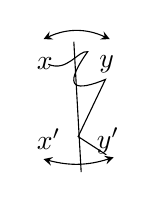
\begin{tikzpicture}[x=.55cm,y=.55cm,>=stealth]
\draw[<->] (-.75,1.65) to[bend left=25] (.78,1.65);
\draw[<->] (-.75,-1.12) to[bend right=16] (.87,-1.08);
\draw (-.05,1.59)--(.12,-1.42);
\draw (-.64,1.07) .. controls (-.2,.88) and (.05,1.4) .. (.27,1.36) .. controls (-.36,.47) and (.02,.45) .. (.68,.72) -- (.05,-.6) -- (.70,-1.02);
\node at (-.72,1.09) {$x$}; \node at (.71,1.08) {$y$};
\node at (-.63,-.65) {$x'$}; \node at (.74,-.70) {$y'$};
\end{tikzpicture}}
est polynomiale (en effet, on aura $\lambda(0)=0\overset{\text{d'où}}{\Longrightarrow}$
$\lambda(\underset{\inserted{\substack{\shortparallel\\0}}}{2x})=2\lambda(x)+\mu(x,x)$, donc $\mu(x,x)=-2\lambda(x)$ \deleted{donc}
$\mu(x,x)\in2Z$ $(\forall x\in V)$, d'où \unsure{facilemt|facilmt|facilement} le
résultat). Donc
\[
\unsure{\mathfrak Z|\mathscr Z}\mathrel{\unsure{=|\subset}} V+
\underset{\displaystyle
 (\mathbb Z/4\mathbb Z)^{(I)}\deleted{+\mathbb Z/4\mathbb Z}
 +(\mathbb Z/2\mathbb Z)^{\mathcal P_2(I)}}{\underbrace{\Gamma_{\mathbb Z}^2(V)}}\unsure{\searrow|\shortparallel}
\]

\hfill TSVP
% archive sheet number: 38
